
\section{SPICE SIMULATIONS}


\subsection{Overview}

LTspice \cite{LTspice} is a simulation software designed to simulate analog electronic circuits. By utilising an equivalent circuit model for a SiPM, it is possible to simulate the features and behaviours of such devices. These results can then be compared to real-world experimental data. The majority of simulations performed were transient analyses, allowing the response of the circuit to be measured based on the arrival of an incident signal.

The resulting output of a LTspice simulation can be exported as a tabulated ASCII file; an example is given in appendix B. These files were then processed using Python and the data graphed using Matplotlib. Some example code is presented in appendix C.

\subsection{Unit Tests}

A initial series of unit tests were performed to ensure: i) familiarity with the different features of the simulation software and ii) it was working as intended and producing sensible results.

\subsubsection{Resistor Circuit}

A DC sweep was performed on a simple resistor circuit (Fig. 3.1) with different resistance values and the resulting IV graph is shown in Fig. 3.2. As expected, we get a linear relationship from Ohm's law.

\begin{figure}[h]
  \centering
  \includegraphics[width=\linewidth]{Graphics/UnitTests/"ResistorCircuit"}
  {\caption*{Fig. 3.1: A simple resistor circuit used in our unit test. The resistor takes values of $10\Omega, 50\Omega$ and $100\Omega$ while the voltage source sweeps through DC values between $-10V$ and $-10V$. The current through the resistor can be measured resulting in the expected IV graph.}}
\end{figure}

\begin{figure}[h]
  \includegraphics[width=\linewidth]{Graphics/UnitTests/"ResistorIVGraph"}
  {\caption*{Fig. 3.2: The resulting IV graph for the resistor circuit.}}
\end{figure}

\subsubsection{RC Circuit}

Two tests were performed on the RC circuit (Fig. 3.3). Firstly, a transient analysis simulates the circuit in the time domain. Using the values in Fig. 3.3, we can see that the charge and current of the capacitor over time is consistent with theory (Fig. 3.4).

Secondly, an AC analysis simulates the response of the circuit in the frequency domain ($V=e^{-i\omega t}$). The resulting Bode plot (Fig. 3.5) shows the frequency dependence of the RC circuit. As expected, the RC circuit acts as a potential divider dependent on frequency. This can also be shown to be consistent with theory analytically using standard circuit rules:

\begin{align*}
  Z &= R-\frac{i}{\omega C} \\
  \left|\frac{V_R}{V_{in}}\right| &= \frac{\omega RC}{\sqrt{1+(\omega RC)^2}}, \phi_R=\frac{\pi}{2}-\tan^{-1}(\omega RC) \\
  \left|\frac{V_C}{V_{in}}\right| &= \frac{1}{\sqrt{1+(\omega RC)^2}}, \phi_C=-\tan^{-1}(\omega RC)
\end{align*}

\begin{figure}[h]
  \centering
  \includegraphics[width=\linewidth]{Graphics/UnitTests/"RCCircuit"}
  {\caption*{Fig. 3.3: A standard RC circuit with $R=1k\Omega$ and $C=1\mu F$. A transient analysis with a DC voltage of $1V$ simulates the charging of the capacitor (Fig. 3.4). An AC analysis with $V=e^{-i\omega t}$ generates a Bode plot between $1Hz$ and $100kHz$. (Fig. 3.5)}}
\end{figure}

\begin{figure}[h]
  \includegraphics[width=\linewidth]{Graphics/UnitTests/"CapacitorTrans"}
  {\caption*{Fig. 3.4: A transient analysis of a RC circuit to simulate capacitor charging. With $R=1k\Omega$ and $C=1\mu F$, we have $\tau=1ms$. We get the expected exponential relationships ($V=1V$): $I=\frac{1}{R}e^{-t/\tau}\to 0A$ and $Q=C(1-e^{-t/\tau})\to 1\mu C$.}}
\end{figure}

\begin{figure}[h]
  \includegraphics[width=\linewidth]{Graphics/UnitTests/"ACAnalyse"}
  {\caption*{Fig. 3.5: An AC analysis of a RC circuit. Using standard circuit rules, we can see the results are in agreement with theory. For example, $\phi_C=-\tan^{-1}(\omega RC)\to -\frac{\pi}{2}$.}}
\end{figure}

\subsection{SPAD Simulation}

\begin{figure}[h]
  \centering
  \includegraphics[width=0.8\linewidth]{Graphics/SPAD/"SPADCircuit"}
  {\caption*{Fig. 3.6: The equivalent SPAD circuit used in the simulations. For convenience, the overvoltage was set to $1V$. The arrival of a photon is simulated by a delta function voltage peak. This voltage peak briefly closes the switch causing the circuit to trigger.}}
\end{figure}

The equivalent circuit model for a SPAD used in our simulations is given in Fig 3.6. With the same approach as \cite{acerbi2019}, we use a switch to simulate the arrival of a photon that triggers the circuit. For our purposes, we model the photon with a voltage signal that activates $10ns$ into the simulation and has a rise/fall time of $0.1ns$. Since these simulations typically run in the region of tens of nanoseconds, we can effectively treat this signal as a delta function. Thus, the voltage signal models a photon impinging on the SPAD which closes the switch and triggers the circuit. An alternative method would be to use a direct current source. \cite{corsi2006}

For convenience, we set the overvoltage to be $1V$ and the other parameters to be typical but idealised values. More realistic values are used when simulating the behaviour of a complete SiPM circuit. There are two main ways we can consider the behaviour of our system: by considering either the current through $R_q$ or the voltage across $C_d$. It was found to be more convenient to measure the current for the most part especially when calculating the recovery time of the SPAD.

Three main sets of simulations were run for the SPAD. Firstly, various parameters in the circuit were varied including $R_q$, $R_d$ and $V_{ov}$ to determine the effect of each component on the resultant signal. Secondly, the effect of various parameters on the SPAD recovery time was studied and compared with theory (Eq. 2.2). Taking the logarithm of the current signal allowed the recovery time to be extracted via a linear regression. Finally, the theoretical value for the gain of a SPAD (Eq. 2.3) was tested by integrating the current to find the total charge. The most significant results are presented in Section 4.1.

\subsection{SiPM Simulation}

\begin{figure*}[h]
  \centering
  \hfill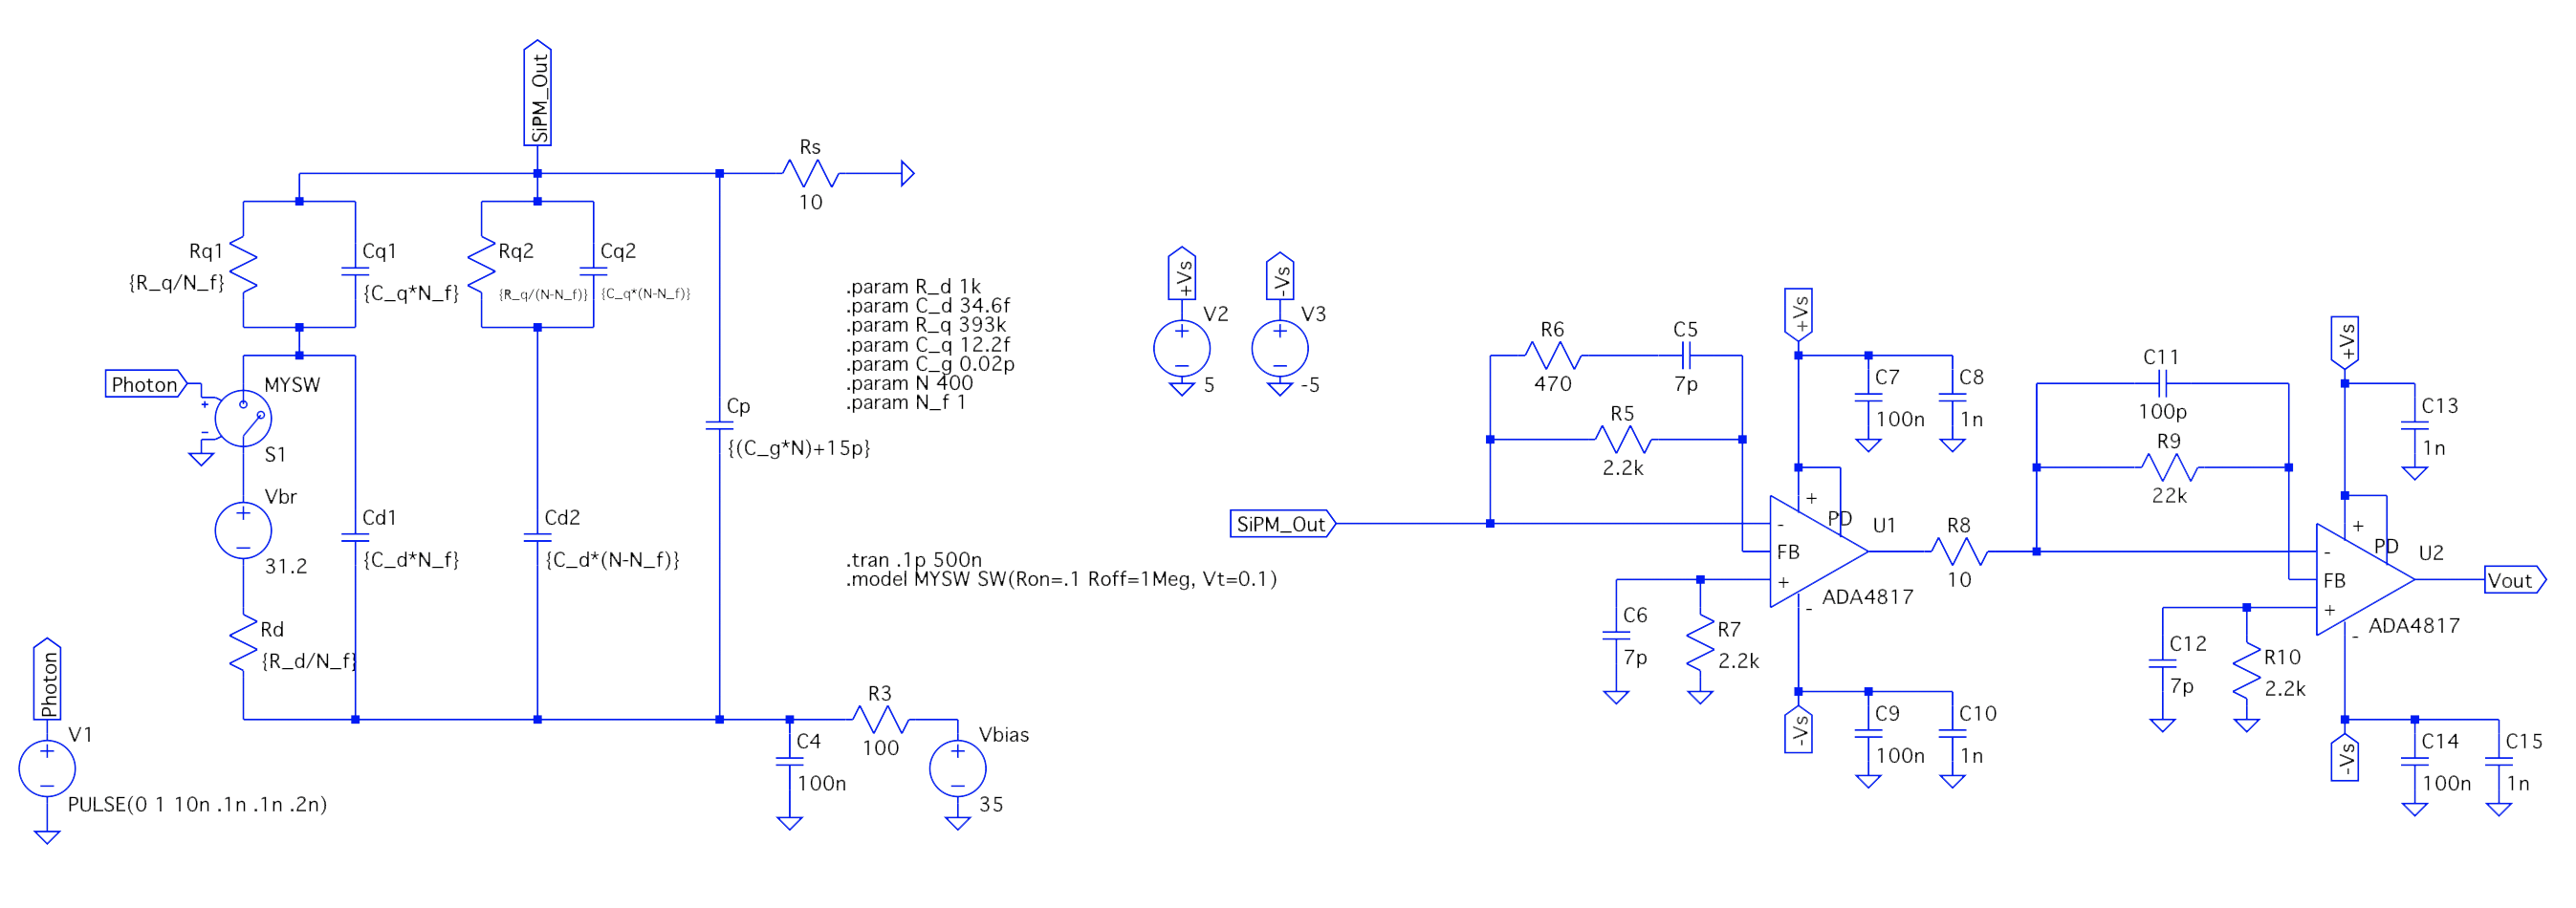
\includegraphics[width=\linewidth]{Graphics/SiPM/SiPMSpice}\hspace*{\fill}
  {\caption*{Fig. 3.7: The complete circuit model used in the simulations. The output of the SiPM is connected to an amplifier circuit based on Fig. 3.8. For most of our simulations, the amplifier was neglected and the voltage signal taken directly from the SiPM output.}}
\end{figure*}

\begin{figure}[h]
  \centering
  \hfill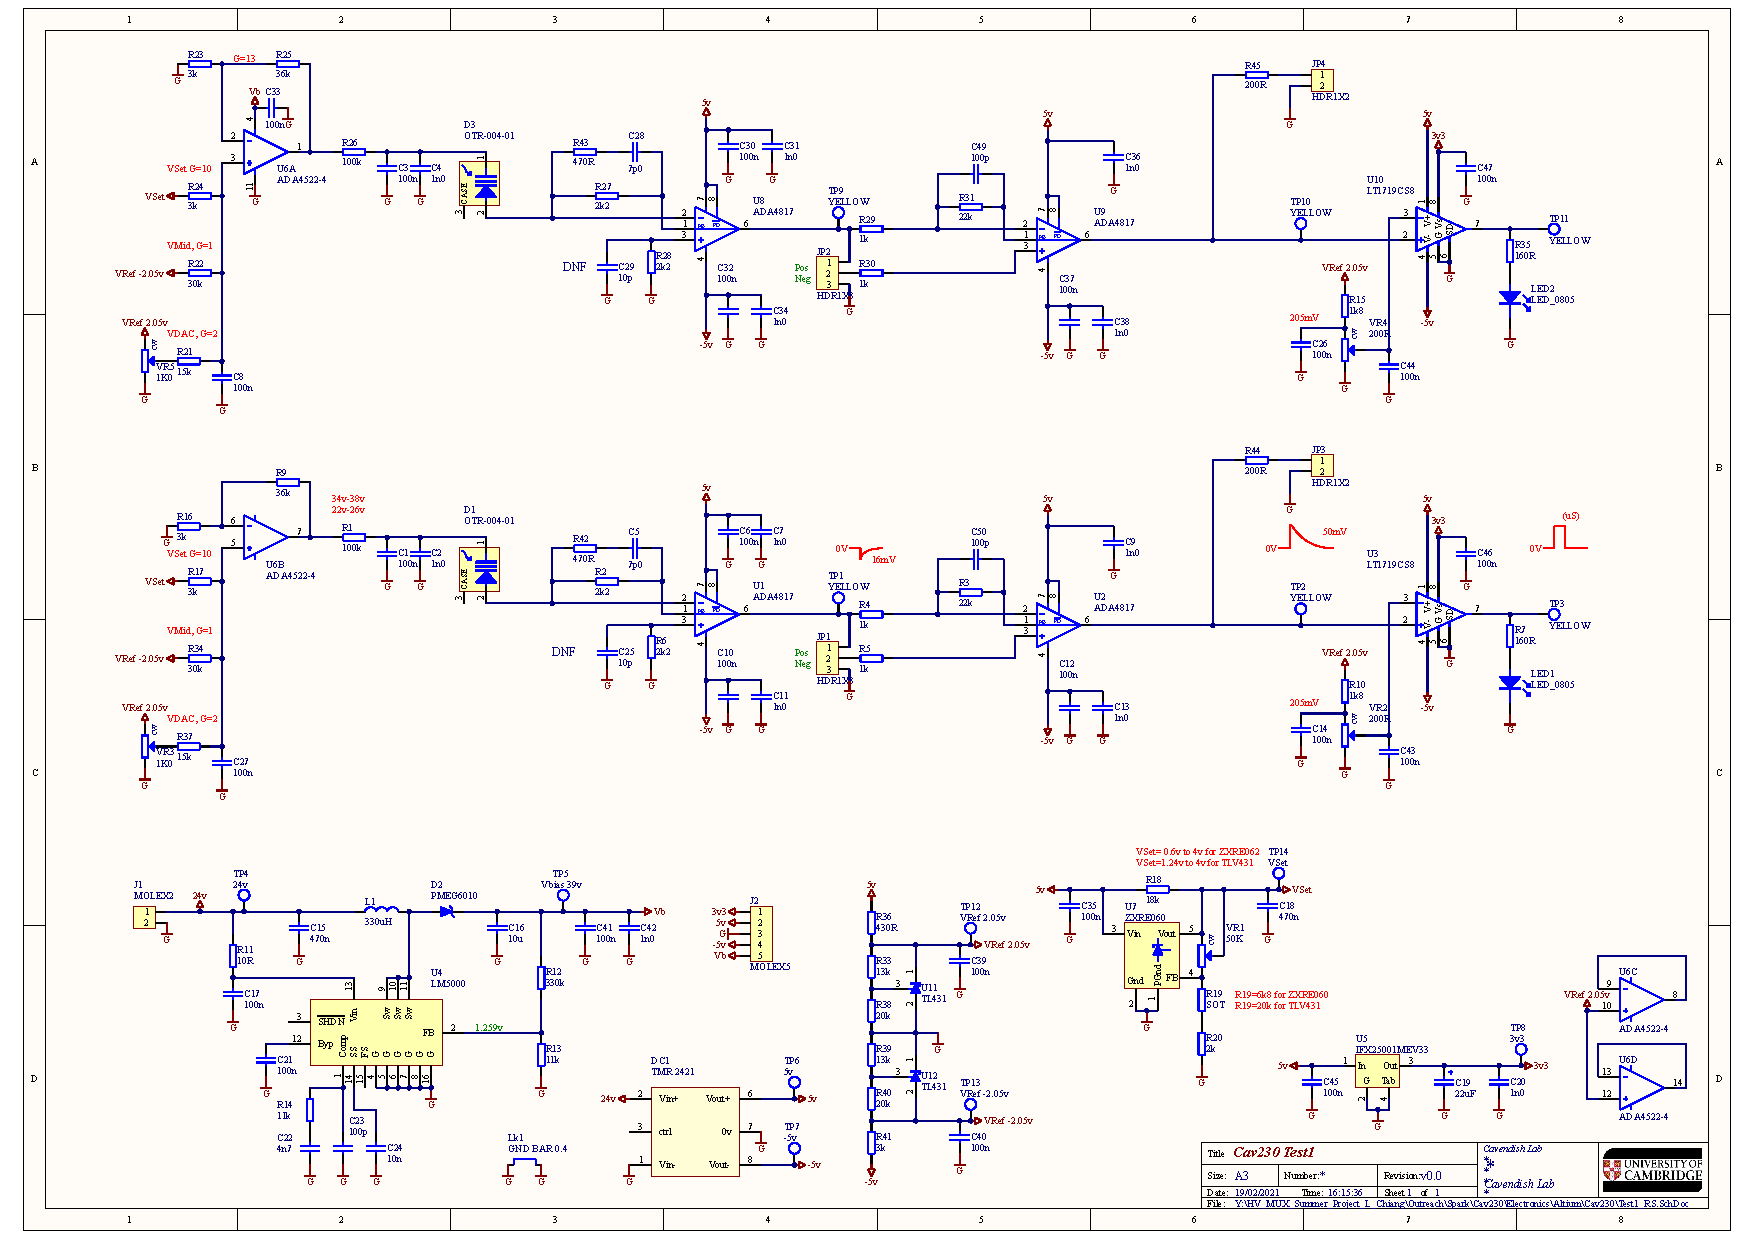
\includegraphics[width=\linewidth]{Graphics/SiPM/AmplifierCircuit}\hspace*{\fill}
  {\caption*{Fig. 3.8: The schematic for the amplifier circuitry that is connected to the SiPMs at the Cavendish Laboratory.}}
\end{figure}

Fig. 3.7 shows the complete SiPM model used in our simulations and is an adaptation to the model used in \cite{acerbi2019}. The output signal of the SiPM is fed into a front-end amplifier based on our current existing experimental setup Fig. 3.8. There are two stages for the amplification process; both of which utilise the $ADA4817$ amplifier \cite{ADA4817amp} to amplify and shape the signal. Note that in the literature, the most common amplifier used in the amplification stage is the $AD8000$. \cite{acerbi2019}\cite{seifert2010} However, for most of our simulations, the amplifier was neglected in favour of taking the final signal directly from the SiPM output.

\begin{table}[h]
\centering
\begin{tabular}{ |c|c|c| }
 \hline
 \textbf{Model} & \textbf{SiPM} & \textbf{SiPM} \\
 \textbf{Parameter} & \textbf{ITC-irst} & \textbf{Photonique} \\
 \hline
 $V_{bias}$ & 35V & 63V \\
 \hline
 $V_{br}$ & 31.2V & 61V \\
 \hline
 $R_{q}$ & 393k\Omega & 774k\Omega \\
 \hline
 $C_d$ & 34.6fF & 40.8fF \\
 \hline
 $C_q$ & 12.2fF & 21.2fF \\
 \hline
 $C_p$ & 27.8pF & 18.1pF \\
 \hline

\end{tabular}
\caption*{Table 1: Adapted from \cite{corsi2006}. The known parameters of two different SiPMs used in our SiPM simulations.}
\end{table}

\noindent In an identical fashion to the SPAD, the model uses a switch to simulate the triggering of the SiPM by a photon. For the model parameters, given that the parameters of our internal laboratory SiPM have not yet been determined, it was decided that values based on 2 known SiPMs should be used. These values are presented in Table 1. Two modifications have been made to this: i) the introduction of a shunt resistor, $R_s$ and ii) allowing the total number of cells in the SiPM to vary. As a result, the parasitic capacitance of the circuit is now given by $C_p=NC_g+15pF$ where $C_g=0.02pF$ - reflecting a greater parasitic capacitance for a larger total number of microcells. In the case of $R_d$, the value was kept at $1k\Omega$ since, as previously mentioned, changing $R_d$ in the range of $\sim 1k\Omega$ doesn't affect the output too much. For our purposes, the SiPM was simulated with $N=400$ and $N=3600$ cells, corresponding to SiPMs of sizes $1\times 1 mm^2$ and $3\times 3 mm^2$ with a $50\mu m$ pitch respectively.

\noindent Similar to the SPAD, a number of different simulations were run. Firstly, the parameters were varied to determine their effects on the voltage signal at the SiPM output. In constrast to the SPAD, there are additional parameters to consider such as the total number of cells ($N$), the total number of fired cells ($N_f$) and the parasitic capacitance ($C_p$). Secondly, the effect of the parameters on the SiPM gain was investigated by taking the integral of the current through $R_s$. We shall see that the gain is now no longer linear due to the additional impedances.

Finally, we use an alternative method to calculate the SiPM microcell recovery time compared to the SPAD case. The subsequent triggering of the circuit simulating the arrival of a photon after the initial one leads to a second output signal. However, if the cell has not fully recovered, the second voltage peak is less than the initial one. We measure the minimum time it takes for the secondary photon to correspond to an output signal that is equal to the initial voltage peak. We also note the time for the secondary signal to be half the size as the initial one.
